\documentclass[../main.tex]{subfiles}
\begin{document}
\onlyinsubfile{
\setcounter{chapter}{8}
}
\notinsubfile{
}
\section{Werken met een echte quantumcomputer}
\onlyinsubfile{
%\marginnote{%\vspace{0cm}
%\textcolor{red}{hoofdstuk is los gecompileerd, hstk nummer is \thechapter}
%}
}
\notinsubfile{
%\marginnote{\vspace{0cm}
%\textcolor{red}{main.tex gecompileerd, nummering zou moeten kloppen}}
}
De quantumcomputer zal in de toekomst niet fysiek in onze telefoons zijn ingebouwd, maar de technologie zal via grote spelers beschikbaar komen. In hoofdstuk~\ref{chap:toepassingen} gaan we op die grote spelers nader in.

\marginpar{\vspace{-3cm}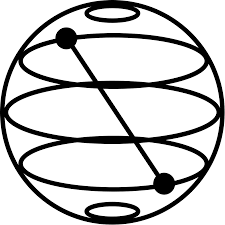
\includegraphics[width=0.95\marginparwidth]{./img/qiskit.png}%\captionof{figure}{Qiskit (IBM). \label {fig:qiskitlogo}}
}
%\marginpar{\vspace{-3cm}
\includegraphics[width=0.95\marginparwidth]{./img/IBM_logo_in.jpg}\captionof{figure}{IBM logo. \label {fig:ibmlogo}}}
\marginpar{\vspace{0cm}
\includegraphics[width=0.95\marginparwidth]{./img/Cirq_logo_color.png}%\captionof{figure}{Cirq (Google). \label {fig:cirqlogo}}
}
\marginpar{\vspace{2cm}
\includegraphics[width=0.95\marginparwidth]{./img/QuantumInpireLogo.png}%\captionof{figure}{QI (TU-Delft). \label {fig:QILogo}}
}
IBM, Google en Qutech hebben quantumcomputers waar ook het publiek gebruik van kan maken. Qutech is misschien minder bekend, maar wel dichtbij. Het is het research instituut van de TU-Delft dat gewijd is aan quantumcomputing. Er staan meer dan tien 'koelkasten'. E\'en daarvan is beschikbaar voor het publiek.

Deze instituten bieden allemaal hun eigen webinterface waarmee een QC bestuurd kan worden, en hebben allemaal prima (Engelstalige) tutorials. de 'koelkasten' zijn ook te besturen met python programma's vanuit je eigen PC. Daarvoor zijn uitgebeide bibliotheken beschikbaar. IBM heeft Qiskit, Google heeft Cirq, en Qutech heeft quantumInpire. Indeze NLT-module gebruiken we \hrefqr{https://www.quantum-inspire.com/}{Quantum Inspire}. 


QI kent twee gebruikersmodi. Zonder een account aan te maken kun je gebruik maken van de simulatie modus. Als je een QC wilt gebruiken moet je een account aanmaken. 
De simulatie mode berekent klassiek, op grond an de wiskunde die we welders in de module gebruiken, de algoritmen door. De klassieke rekenkracht die nodig is voor simulaties neemt exponentieel toe met het aantal qubits. De simulatiemode van QI is beperkt tot vijf qubits, Ruim voldoende voor onze toepassingen.
Met een knipoog naar het eerste programma dat je in een nieuwe computertaal schrijft heet dit programma "hello quantumworld". In de knowledge base wordt het programma regel voor regel beschreven.
[NB aug 2020 links op de pagina werken niet]

Twee qubits, q[0] en q[1], worden ge\"initialiseerd in de grondtoestand $\ket{0}$. 


\begin{antwoord}
\end{antwoord}
\begin{opdracht}
Lees de tekst in the knoledge base (engels) over het startprogramma. Daarin wordt het programma regel voor regel uitgelegd. Beantwoord daarna de volgende vragen. Start de \href{https://www.quantum-inspire.com/}{demo editor} vanuit de startpagina. 


Kun je voorspellen wat het antwoord is? Natuurlijk heb je al op run
\end{opdracht}

Als je een programma niet afsluit met een meetblikje berekent de simulator in bijna alle gevallen de statistische kansverdeling.

Als je een progamma wel beeindigt met een meting wordt er een trekking uitgevoerd.

\begin{center}
\leavevmode
\Qcircuit @C=1em @R=2em {
\lstick{q[0]} & \ustick{\ket{0}} & \qw &\gate{H} & \ctrl{1} & \qw & \qw & \ustick{\ket{x}}& \rstick{control}\\
\lstick{q[1]} & \ustick{\ket{0}}& \qw &\qw       & \targ & \qw & \qw & \ustick{\ket{x}} & \rstick{target}
}
\end{center}


\end{document}.

